\documentclass{article}
% enable Chinese Characters
\usepackage{ctex}
% calligraphy characters (English)
\usepackage{calligra}
% colored test
\usepackage{xcolor}
% writing paths
\usepackage{url}
% math packages
\usepackage{amsmath, amssymb, amsthm}
\usepackage{mismath}
% plotting graphs
\usepackage{pgfplots}
% pseudocode
\usepackage{algpseudocodex}
% image packages
\usepackage{graphicx, float}
\graphicspath{{images/}}
\parindent 0px

\title{数学建模参考}
\author{Ray Xia}
\date{2025/07/05}

\begin{document}

\maketitle

\tableofcontents

\newpage


\section{前言 \calligra{Forward}}

本文作为数学建模的非权威性参考资料,主要包含了针对全国大学生数学建模大赛(国赛)
的相关参考资料,以便翻阅查找。
程序编写主要采用python语言,使用的主要库有:

\begin{itemize}
    \item[numpy, pandas] 无需多盐
    \item[pulp] 线性规划
    \item[sklearn] 大部分经典算法
    \item[keras] 神经网络
    \item[matplotlib] 绘图
    \item[pymoo] 多目标优化
    \item[pygad] 遗传算法
\end{itemize}

程序的编写标准基于Google Python Style Guide进行调整:

\begin{enumerate}
    \item 执行类文件(.ipynb)中禁止使用异常处理,所有函数在\textbf{输入正确的情况下}都用该成功返回。非执行类文件中可以简单使用(如检测参数是否正确等)。
    \item 所有执行类文件以Jupyter Notebook(.ipynb)形式;非执行类文件(库,配置文件)都使用.py形式。
    \item 所有执行类文件都应该能够从头到尾运行一次,并得到正确结果(不要依赖特殊的Jupyter Notebook的执行顺序)。
        使用Jupyter Notebook只是为了方便编写调试。
\end{enumerate}


\section{数学基础 \calligra{Mathemathical Fundamentals}}

\begin{itemize}
    \item[高等数学] 包含一(多)元函数极限、一(多)元函数微分学,一(多)函数积分学、等
    \item[线性代数] 矩阵、特征值、等
    \item[概率统计] 作者也没有学过,但是马尔科夫链等模型应该和这个有点关系。只是理解模型的话,高中的知识就足够了。
\end{itemize}

\section{符号与惯用标记 \calligra{Notations}}

\hbox{
\begin{tabular}{ll}
\hline
Notation & Meaning \\ \hline
\(x, y, z\)  & Generic Variables\\
\(f, g, h\) & Generic Functions\\
\(\mathbf{x_n, y_n, z_n}\)  & Vector Variables with a dimension of \(n\)\\
\(\mathbf{f_n, g_n, h_n}\)  & Vector Functions with a dimension of \(n\)\\
\(\mathbf{A, B, M},\begin{bmatrix}
    1 & 0 \\ 0 & 1
\end{bmatrix}\) & Matrices \\
\(\mathbf{M}^T\) & Transposed Matrices \\
\(\mathbf{a} >(<, \geqslant, \leqslant) \mathbf{b}\) & \(\forall a_i > (<, \geqslant, \leqslant) b_i\) \\
\(\lVert\mathbf{x}\rVert_n\) & $\mathbf{x}$的$n$范数, 如果是二范数则可以省略$n$\\
$A := B$ & 定义$A$为$B$ \\
\end{tabular}
}

如果没有特殊说明,所有向量都是列向量。


\section{常用模型/算法 \calligra{Common Models / Algorithms}}

此部分包含了数学建模中常用的一些模型或算法。

根据模型/算法的用途,可将其分为:

\begin{itemize}
    \item{优化算法}
        \[\begin{split}
            &minimize\;\mathbf{x},\\
            s.t.\;&\mathbf{F}(\mathbf{x}) = 0
        \end{split}\]
    \item{预测算法}
        \[\begin{split}
            \text{history data} \stackrel{algorithm}{\Rightarrow} \text{experience (model)} \Rightarrow \text{prediction}
        \end{split}\]
    \item{评价算法}
        \[\begin{split}
            \text{data} \stackrel{\text{(standard)}}{\Rightarrow} \text{scoring}
        \end{split}\]
    \item{其他} 权重决策(重要性分析)
\end{itemize}

每个部分除特殊情况都应该包含一下要点:

\subsection{示例 Example}

这是该模型/算法的基本介绍。

\begin{itemize}

\item{原理}

这是更为详细的原理解释。

\begin{equation}
    \begin{split}
        &\text{可能还会附带一些数学推理/公式和插图。}\\
        & x = 1 + 1 \\
        & x = 2 \\
    \end{split}
\end{equation}

\begin{figure}[H]
    \centering
    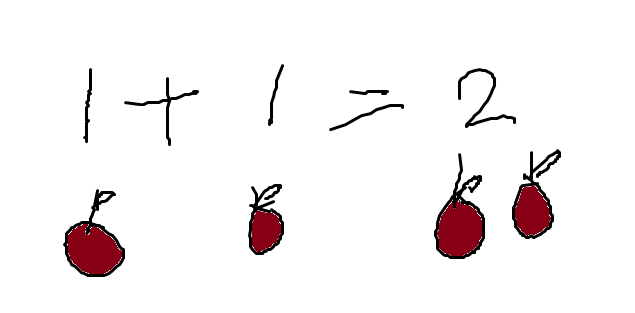
\includegraphics[width = 3in]{placeholder}
    \caption{placeholder}
    \label{fig:placeholder}
\end{figure}

\item{特性}

这是算法特性的基本介绍。

\begin{itemize}
    \item (优点)
    \item (缺点)
    \item (适用场景)
    \item (其他)
\end{itemize}

\item{python 代码实现}

\begin{verbatim}
if __name__ == "__main__":
    print("hello world")
\end{verbatim}

\end{itemize}

根据模型/算法的用途,可将其分为:

\begin{itemize}
    \item[优化算法]
        \[\begin{split}
            &minimize\;\mathbf{x},\\
            s.t.\;&\mathbf{F}(\mathbf{x}) = 0
        \end{split}\]
    \item[预测算法]
        \[\begin{split}
            \text{history data} \stackrel{algorithm}{\Rightarrow} \text{experience (model)} \Rightarrow \text{prediction}
        \end{split}\]
    \item[评价算法]
        \[\begin{split}
            \text{data} \stackrel{\text{(standard)}}{\Rightarrow} \text{scoring}
        \end{split}\]
    \item[其他] 权重决策(重要性分析)
\end{itemize}

需要注意的是:
\begin{enumerate}
    \item 每个部分的算法都大致按照算法的使用率/优先程度从高到低排列。
    \item 部分算法可能会有多个用途,为了避免重复,这些算法在全文中只会出现一次。
\end{enumerate}

\subsection{优化算法}

\subsubsection{线性规划(单目标) Linear Programming}

\url{https://en.wikipedia.org/wiki/Linear_programming}

最基本的有约束的优化问题,更加复杂的形式包含整形规划(Integer Programming)
此部分只讨论单目标规划的情况。

\begin{itemize}

\item{原理}

限制条件的并集会会形成一个可行域,最优解必然出现在该可行域的边界上。

\begin{equation}
    \begin{split}
        \min &\; \mathbf{c}^T\mathbf{x} \\
        s.t. &\; \mathbf{Ax} \leqslant \mathbf{b} \\
    \end{split}
    \;\stackrel{or}{\Leftrightarrow}\;
    \begin{split}
        find\,\min \{\mathbf{c}^T\mathbf{x} | \mathbf{Ax} \leqslant \mathbf{b}\}
    \end{split}
\end{equation}

\item{特性}

线性规划可以说是最简单的一个优化算法了。

\begin{itemize}
    \item 简单,找到的必定是全局最优解。
    \item 需要把条件转化成可以计算的数学条件,只能用于线性的条件。
    \item 适用于简单,孤立的问题。
\end{itemize}

\item{python 代码实现}

线性规划使用的是python的pulp库。

示例可见\path{src/linear_programming/main.ipynb}
g'g
\end{itemize}

\subsubsection{遗传算法 Genetic Algorithm}

通过变异、选择的方式优化问题。

\begin{itemize}

\item{原理}

目标:

\begin{equation}
    \begin{split}
        \min &\, \Phi(\mathbf{x}) \\
        & \text{, where $\Phi$ is an unknown or overly complex function}\\
        s.t. &\, \mathbf{Ax} \leqslant \mathbf{b}\\
    \end{split}
\end{equation}

\begin{enumerate}
    \item 初始化一个参数随机的种群。
    \item 用函数检测每个个体的适应程度。
    \item 适应程度高的个体被选为父本。
    \item 父本之间结合生成新个体。
    \item 新个体发生变异。
    \item 新个体取代种群中的部分个体。
    \item 重复 2-6 步。
\end{enumerate}

\item{特性}

遗传算法比较简单粗暴,效率比较低下,说不出来什么名道,不建议使用。

\begin{itemize}
    \item 黑盒化对待,不需要知道目标函数的具体形式,只需要输入和输出。
    \item 得到的可能是局部最优;参数选择对最后结果有很大影响。
\end{itemize}

\item{python 代码实现}

使用的是pygad库。

\url{https://pygad.readthedocs.io/en/latest/index.html}

示例见\path{src/genetic_algorithm/main.ipynb}

\end{itemize}

\subsubsection{多目标遗传优化算法 NSGA-II}

GA + 多目标优化来获得一个区间内的 Pareto Front.

\begin{itemize}

\item{原理}

多目标优化中遗传算法的选择标准(non-dominated sorting):

\begin{equation}
    \begin{split}
        & \text{Given an objective function of multiple dimensions to \textbf{minimize}: $\mathbf{F}$}. \\
        & \text{And $X$ is the set of the whole population.}\\
        & \widetilde{F_1} = \{\mathbf{x} | \mathbf{x} \in X \land ( \exists \mathbf{x}_0\in X \,(\mathbf{F}(\mathbf{x}) > \mathbf{F}(\mathbf{x}_0))) \}, \\
        & \widetilde{F_i} = \{\mathbf{x} | \mathbf{x} \in X - \bigcup_{k = 1}^{i - 1} F_k \land ( \exists \mathbf{x}_0\in X- \bigcup_{k = 1}^{i - 1} F_k \,(\mathbf{F}(\mathbf{x}) > \mathbf{F}(\mathbf{x}_0))) \}. \\
    \end{split}
\end{equation}

\item{特性}

说不出来什么名道,不建议使用。

\begin{itemize}
    \item 黑盒化对待,不需要知道目标函数的具体形式,只需要输入和输出。
    \item 复杂;得到的是一组Pareto Front,还需要进一步选出最优方案。
\end{itemize}

\item{python 代码实现}

使用的是pymoo库。\url{https://pymoo.org/algorithms/moo/nsga2.html}
% 示例见\path{src/NSGA-II/main.ipynb}

\end{itemize}
\subsubsection{蚁群算法 Ant Colony Optimization}

\subsubsection{模拟退火 Simulated Annealing}

\newpage



\subsection{预测算法}

\subsubsection{线性回归 Linear Regression}

用一个一次函数拟合多个样本点,目标是使预测结果和样本点的方差最小。

\begin{itemize}

\item{原理}

\begin{equation}
    \begin{split}
        & \text{假设样本点为$\mathbf{x}_0 \mapsto \mathbf{y}_0$}  \\
        &\min_\mathbf{A, b} \, \lVert \mathbf{Ax}_0 + \mathbf{b} - \mathbf{y}_0 \rVert \\
    \end{split}
\end{equation}

\item{特性}

对线性特征明显,无大幅度波动的数据表现良好。

\begin{itemize}
    \item 简单、可解释。
    \item 只适用于线性性良好的数据。
\end{itemize}

\item{python 代码实现}

用的是scikit-learn库\\
示例见\path{linear_models\linear_regression.ipynb}
注意reshape。

\end{itemize}

\subsubsection{线性回归ultra(岭、Lasso、弹性网回归)\\ Ridge, Lasso, Elastic-Net Regression}

岭回归、Lasso、弹性网回归是为了减少数据波动对得回归函数的影响。

\begin{itemize}

\item{原理}

这三种回归在线性回归的基础上增加了不同的规范函数($\alpha,\rho$都是参数):

\begin{equation}
    \begin{split}
        \text{线性回归:} &\\
        &\min\,\lVert \mathbf{Ax + b - y_0}\rVert_2\\
        \text{岭回归:} &\\
        &\min\,\lVert \mathbf{Ax + b - y_0}\rVert_2^2 + \alpha \lVert \mathbf{A} \rVert^2\\
        \text{Lasso回归:} &\\
        &\min\, \frac{\lVert \mathbf{Ax + b - y_0}\rVert_2^2}{2n_{\text{samples}}} + \alpha \lVert \mathbf{A} \rVert_1\\
        \text{弹性网回归:} &\\
        &\min\, \frac{\lVert \mathbf{Ax + b - y_0}\rVert_2^2}{2n_{\text{samples}}} + \alpha\rho\lVert\mathbf{A}\rVert_1 + \frac{\alpha(1 - \rho)}{2} \lVert \mathbf{A} \rVert_2^2\\
    \end{split}
\end{equation}

$\alpha, \rho$确定方法:
\begin{enumerate}
    \item Cross Validation
    \item Akaike Information Criterion / Bayes Information Criterion
\end{enumerate}

\item{特性}

\begin{itemize}
    \item  适合拟合波动较大的数据。
    \item  要确定合适的规范参数($\alpha, \rho$)。
    \item  建议在普通线性回归无法良好拟合的时候使用。
\end{itemize}

\item{python 代码实现}

建议先将数据正规化(normalize)或标准化(standardize)再进行拟合。

示例见\path{src/linear_models/ridge_regression.ipynb}\\
\path{src/linear_models/Lasso_regression.ipynb}\\
\path{src/linear_models/elastic-net_regression.ipynb}\\

\end{itemize}

\subsubsection{随机森林 Random Forest}

bagging算法+决策树+voting

\begin{itemize}

\item{原理}

将数据随机分组,用来训练多个单独的决策树,预测的时候所有决策树的投票。

\begin{algorithmic}
\Procedure{Train}{TrainingData}
    \ForAll{DecisionTree $\in$ Forest}
        \State TrainingDataSet $\subset$ TrainingData
        \State DecisionTree $\rightarrow$ \Call{Fit}{TrainingDataSet}
    \EndFor
\EndProcedure
\Procedure{Predict}{Input}
    \State Votes
    \ForAll{DecisionTree $\in$ Forest}
        \State DecisionTree $\rightarrow$ \Call{Vote}{Input}
    \EndFor
    \Return $\max$ Votes
\EndProcedure
\end{algorithmic}

\item{特性}

主要是解决了决策树容易过拟合的问题。

\begin{itemize}
    \item  快。
    \item  不适合维度很高的数据集;只建议用来预测在输入数据范围内的数据点,不太能预测显著在样本范围之外的数据点。
\end{itemize}

\item{python 代码实现}

示例见\path{src\decision_tree\random_forest.ipynb}

\end{itemize}

\subsubsection{自回归综合移动平均 ARIMA}

时间序列模型:自回归+综合+移动平均。

\begin{itemize}

\item{原理}

自回归、综合、移动平均分别的原理:

\begin{equation}
    \begin{split}
        \text{AutoRegression(\bf{AR})(p):}&\\
        & y_t = \boldsymbol{\phi}^T\mathbf{y}_{t-1 \sim t-p} + c + \epsilon_t\\
        \text{Integrated(\bf{I})(d):}&\\
        & \text{find } d \in \mathbb{N} \text{ so that}\\
        & \{y_n\} \text{ is a $d^{th}$ order arithmatic sequence.}\\
        & \text{(d阶等差数列)}\\
        \text{MovingAverage(\bf{MA})(q)}&\\
        & y_t = \mu + \boldsymbol{\theta}^T\boldsymbol{\epsilon}_{t - 1 \sim t - q} + \epsilon_t
    \end{split}
\end{equation}

其中$\mathbf{y}_{i \sim j}$表示从第$i$个到第$j$个的样本点;
$\boldsymbol{\phi}, \boldsymbol{\theta}, c, \mu$表示有待优化的变量;
$\epsilon_t$表示第$t$次预测的误差。

所以整个ARIMA时间序列模型有三个参数:$p, d, q$需要在拟合之前确定,也可以用Auto ARIMA让算法自动确定这些参数。

\item{特性}

结合了三种算法,能够辨识数据中的整体变化趋势、周期性。

\begin{itemize}
    \item  准确度高,可解释性强。
    \item  手动确定参数有一定技术含量。
    \item  时间序列模型的标杆。
\end{itemize}

\item{python 代码实现}

示例见\path{src\time_series\ARIMA.ipynb},\\
\path{src\time_series\AutoARIMA.ipynb}

\end{itemize}
\subsubsection{马尔科夫链/预测 Markov Prediction Model}

使用(多次)条件概率的方式预测未来某个状体的可能性。

\begin{itemize}

\item{原理}

假设某个事件总共有有限个可能状态:$\{A_1, A_2, A_3, \ldots, A_n\}$,且同时有且仅有一个状态发生。

现在有$T$次历史发生过的状态的记录:$\{A_{i_1}, A_{i_2}, \ldots, A_{i_T}\}$。

那么$A_{i}$发生之后紧接着发生$A_{j}$的频率为:

\[f_{j, i}:=\mathbf{f}(A_j \mid A_i) = \frac{N_{A_i \rightarrow A_j}}{N_{A_i \rightarrow any}}\]

显然有:

\[(\forall i \in [1, n])\left(\sum_{j = 1}^{n} f_{j, i} = 1\right)\]

如果\textbf{把频率作为概率},那么就得到了状态转移的概率矩阵:

\[\mathbf{P}_{n\times n} = \begin{bmatrix}
    p_{1, 1} & p_{1, 2} & \cdots & p_{1, n}\\
    p_{2, 1} & p_{2, 2} & \cdots & p_{2, n}\\
    \vdots & \vdots & \ddots  & \vdots\\
    p_{n, 1} & p_{n, 2} & \cdots & p_{n, n}\\
\end{bmatrix} = [f_{i, j}] = \begin{bmatrix}
    f_{1, 1} & f_{1, 2} & \cdots & f_{1, n}\\
    f_{2, 1} & f_{2, 2} & \cdots & f_{2, n}\\
    \vdots & \vdots & \ddots  & \vdots\\
    f_{n, 1} & f_{n, 2} & \cdots & f_{n, n}\\
\end{bmatrix}\]

假设最近一次的状态为$A_i$,那么下一次每个状态发生的概率为:

\[\mathbf{p}_1 := \begin{bmatrix}
    \mathbf{P}(A_1)\\
    \mathbf{P}(A_1)\\
    \vdots\\
    \mathbf{P}(A_1)\\
\end{bmatrix} = \begin{bmatrix}
    \mathbf{P}(A_1 \mid A_i)\\
    \mathbf{P}(A_1 \mid A_i)\\
    \vdots\\
    \mathbf{P}(A_1 \mid A_i)\\
\end{bmatrix} = \mathbf{P}\times\begin{bmatrix}
    0\\
    \vdots\\
    1_\text{(i-th element)}\\
    \vdots\\
    0\\
\end{bmatrix} = \mathbf{P} \times \mathbf{e}_i\]

后面第$k$次,每个状态发生的概率为:

\[\mathbf{p}_k :=\begin{bmatrix}
    \mathbf{P}(A_1)\\
    \mathbf{P}(A_1)\\
    \vdots\\
    \mathbf{P}(A_1)\\
\end{bmatrix} = normalized(\mathbf{P}^k\times \mathbf{e}_i)\]

让$k\rightarrow \infty$可以得到整体的发展趋势:

\[\mathbf{p} := \lim_{k\rightarrow \infty}\mathbf{p}_k = \mathbf{P}^\infty \times \mathbf{e}_i\]

\item{特性}

就业场景较为狭窄。

\begin{itemize}
    \item  可解释性强,使用简单。
    \item 非常粗糙地假设每次状体只与前一次的状态有关。
\end{itemize}

\item{python 代码实现}

实现见:\path{src/probabilities/markov_model.py}\\
示例见:\path{src/probabilities/markov_model.ipynb}

\end{itemize}

\subsubsection{梯度提升树 Gradient Boosting Trees}

除了随机森林的另一种基于决策树的拟合算法。

\begin{itemize}

\item{原理}

用一个新的决策树去拟合已有模型的误差,在整合到模型当中。

\begin{algorithmic}
\Procedure{Train}{TrainingData}
    \Repeat
    \State Errors $\leftarrow$ (Model $\rightarrow$ \Call{Errors}{TrainingData})
    \State NewTree $\rightarrow$ \Call{Fit}{Errors}
    \State Model += NewTree
    \Until{N Trees in Model}
\EndProcedure
\end{algorithmic}

\item{特性}

\begin{itemize}
    \item 准确度高,可解释性强。
    \item 拟合比较缓慢;要确定合适的参数(决策树的数量)来防止过拟合。
\end{itemize}

\item{python 代码实现}

对样本数量比较少的情况($<10,000$)建议使用 GradientBoostingClassifier / GradientBoostingRegressor\\
对样本数量比较多的情况($>10,000$)建议使用 HistGradientBoostingClassifier / HistGradientBoostingRegressor

示例见\path{src/decision_tree/gradient_boosting.ipynb}

\end{itemize}

\subsubsection{灰色预测 Grey Method}

一种通过累加使数据趋势更加明显后,再进行预测的预测算法。

\begin{itemize}

\item{原理}

通过求和(或积分)使数据趋势更加明显。

假设数据$x$是连续的,$X$是其原函数(为了方便这里讨论的是一维数据):

\[X = \int_{0}^{t}x\di t\]

假设$\mathbf{X}$满足常微分方程,也就是满足指数关系:

\[\begin{split}
    \frac{\di X}{\di t} + aX & = b\\
    \Leftrightarrow X & = \frac{b}{a} + Ce^{-ax}\\
    \Rightarrow x = \frac{\di X}{\di t} & = -aCe^{-ax}\\
\end{split}\]

现在的问题就是如何得到合适的参数$a, b, C$。

假设有$x$在$t_0, t_1, \ldots, t_n$时刻的数据$x(t_0), x(t_1),\ldots, x(t_n)$。
那么可以估计$X$在对应时刻的数值(假设$t_0=0$):

\[\begin{split}
X(t_i) & = \int_{0}^{t_i}x\di t\\
& = \sum_{k = 0}^{i - 1}\int_{t_k}^{t_{k + 1}} x \di t\\
& \approx \sum_{k = 0}^{i - 1}\frac{1}{2}(x(t_k) + x(t_{k + 1}))(t_{k + 1} - t_k)\\
\end{split}\]

有了$x, X$就可以用最小二乘法求出常微分方程中的$a, b$,再对$X$的解析式用一次最小二乘,来求得合适的$C$。

\item{特性}

\begin{itemize}
    \item 非常简单,可解释性强;对噪声有一定屏蔽能力。
    \item 对异常值应对能力差;长期预测能力差。
    \item 适用于样本点较少的情况。
\end{itemize}

\item{python 代码实现}

\path{src/grey_model/gm_1_1.py}

示例见\path{src/decision_tree/main.ipynb}

\end{itemize}

\subsubsection{朴素贝叶斯 Naive Bayes}

一种基于贝叶斯理论的预测模型。

\begin{itemize}

\item{原理}

贝叶斯模型假设自变量之间都是独立的。

\[\begin{split}
P(y \mid x_1 x_2 \ldots x_n) & = \frac{P(y \land x_1 x_2 \ldots x_n)}{P(x_1 x_2 \ldots x_n)}\\
& = \frac{P(y)P(x_1 x_2 \ldots x_n \mid y)}{P(x_1 x_2 \ldots x_n)}\\
\end{split}\]

因为$x_i$之间都是独立的,所以有:

\[\begin{split}
P(y \mid x_1 x_2 \ldots x_n) & = \frac{P(y)\prod_{i=1}^{n}P(x_i \mid y)}{P(x_1 x_2 \ldots x_n)}\\
\end{split}\]

\[\begin{split}
    \Rightarrow E(y) & = \arg \max_y P(y \mid x_1 x_2 \ldots x_n) \\
    & = \arg \max_y \frac{P(y)\prod_{i=1}^{n}P(x_i \mid y)}{P(x_1 x_2 \ldots x_n)} \\
    & \stackrel{P(x_1 x_2 \ldots x_n) = C(y)}{=} \arg \max_y \left[P(y)\prod_{i=1}^{n}P(x_i \mid y)\right] \\
\end{split}\]

\item{特性}

\begin{itemize}
    \item 非常简单,可解释性强;速度很快。
    \item 精度较低;在实际情况中假设不一定成立。
\end{itemize}

\item{python 代码实现}

示例见\path{src/probabilities/naive_bayes.ipynb}

\end{itemize}

\subsubsection{决策树 Decision Tree}

\begin{itemize}

\item{原理}

通过增加分支和判断条件得出预测结果。

\begin{figure}[H]
    \centering
    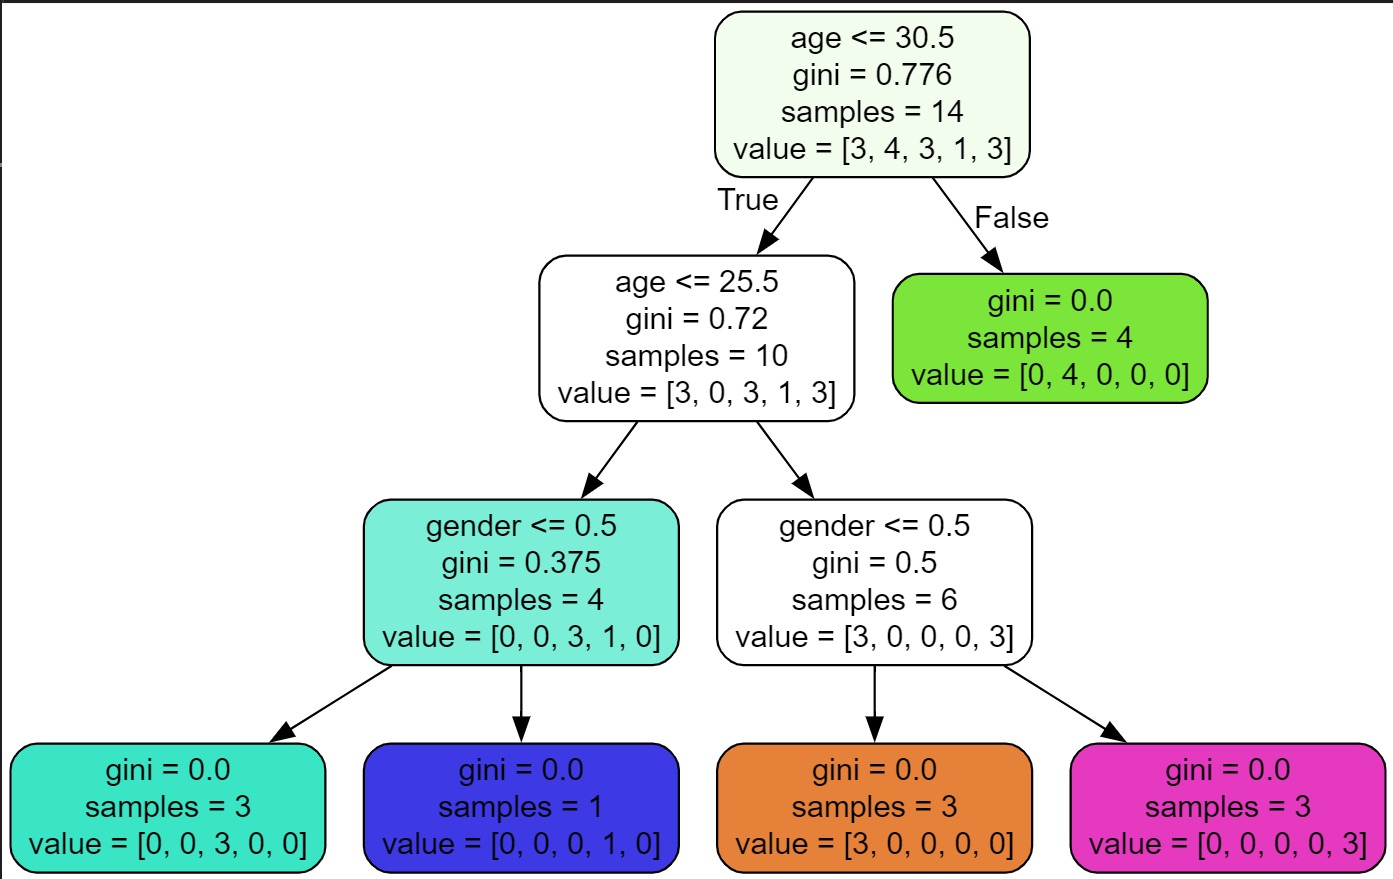
\includegraphics[width = 3in]{decision_tree}
    \caption{决策树示意图}
    \label{fig:decision_tree}
\end{figure}

\item{特性}

\begin{itemize}
    \item 非常简单,可解释性强;速度很快。
    \item 容易受噪声影响;容易过拟合。
\end{itemize}

\item{python 代码实现}

示例见\path{src/decision_tree/decision_tree.ipynb}

\end{itemize}

\subsubsection{K近邻 K-Nearest Neighbours}

根据预测点周围最近的$K$个样本点的标签确定预测标签。

\begin{itemize}

\item{原理}

通过增加分支和判断条件得出预测结果。

对于数据集$S$中的样本点和对应的标签:$(x, y)$。
对于预测点$\hat{x}$:

\[\begin{split}
    N:\; & (N \subset S) \land (|N| = k) \land\\
    & (\forall (x, y) \in N, (x', y') \in S \backslash  N)(\lVert x - \hat{x} \rVert < \lVert x' - \hat{x} \rVert)\\
\end{split}\]

预测结果$\hat{y}$为$N$中出现次数最多的数据点(也可以用距离作为权重进行累加)。

\item{特性}

\begin{itemize}
    \item 参数k的确定对模型的准确性影响很大;对噪声和异常值敏感;容易过拟合或者拟合不良;对较大的数据集速度慢。
\end{itemize}

\item{python 代码实现}

示例见\path{src/k_nearest_neighbors/main.ipynb}

\end{itemize}

\subsubsection{K均值聚类 K-Means Clustering}

非监督学习聚类算法。

\begin{itemize}

\item{原理}

\begin{algorithmic}
\Procedure{Train}{DataPoints}
    \State Randomly select Centroids
    \Repeat
    \State DataPoints $\rightarrow$ closest Centroid
    \State Centroids = \Call{Mean}{data points}
    \Until{Centroids stop changing}
\EndProcedure
\end{algorithmic}

\item{特性}

\begin{itemize}
    \item 聚类数k必须预先确定;对于线性性较差的数据集表现较差。
\end{itemize}

\item{python 代码实现}

示例见\path{src/k_means_clustoring/main.ipynb}

\end{itemize}

\subsubsection{支持向量机 Support Vector Machine}

通过构造一个超平面,再通过计算样本点到超平面的距离来确定预测结果。

\begin{itemize}

\item{原理}

假设样本是$n$维的数据集,预测标签只有两种类型。
可以尝试在样本的$n$维空间中找出一个超平面,使该平面将不同标签的样本点分布在平面的两侧,并使不同样本点离平面的距离最大。

几个常见的问题和解决方法:
\begin{itemize}
    \item{样本点不是线性可分的}
    \begin{itemize}
        \item{近似线性可分}
            设置一定宽容度,使得距离在这个范围内的样本点可以分布在超平面的任意一侧。
        \item{完全不线性可分}
            添加核函数(Kernel Function)改变样本点在空间中的分布形态。
    \end{itemize}
    \item{有多种($>2$)预测标签}\\
        假设有$m$种不同的标签,可以使用以下策略:
        \begin{itemize}
            \item{One versus One} 创建$\frac{m(m - 1)}{2}$个SVM模型。
            \item{One versus Rest} 创建$m$个SVM模型。
        \end{itemize}
\end{itemize}

\item{特性}

\begin{itemize}
    \item 可解释性强;找到的支持向量\textbf{可能}有实际意义;适用于样本维度大于样本数的情况。
    \item 对样本数很大的数据集表现较差。
\end{itemize}

\item{python 代码实现}

示例见\path{src/support_vector_machine/main.ipynb}

\end{itemize}

\subsubsection{神经网络 Neural Network}

基本的神经网络(MLP)。

\begin{itemize}

\item{原理}

一个神经网络由多个层构成,每一层由多个节点组成,每个结点的值都是前一层所有结点分别的仿射变换套上一个激活函数。

记$n_{i, j}$为第$i$层的第$j$个节点,那么有:

\[\begin{split}
    n_{i + 1, j} = \sum_j \left[a_{(i, k) \rightarrow (i + 1, j)}n_{i, k} + b_{(i - 1, k) \rightarrow (i + 1, j)}\right]
\end{split}\]

\item{特性}

\begin{itemize}
    \item 可解释性强;找到的支持向量\textbf{可能}有实际意义;适用于样本维度大于样本数的情况。
    \item 对样本数很大的数据集表现较差。
\end{itemize}

\item{python 代码实现}

示例见\path{src/support_vector_machine/main.ipynb}

\end{itemize}

\subsubsection{逻辑斯谛回归 Logistic Regression}

\subsubsection{密度聚类 DBSCAN}

\subsubsection{卷积神经网络 Convolutional Neural Network}

\subsection{评价算法}

\subsubsection{优劣解距离法 TOPSIS}

基于相对最优\&最差方案的距离进行评价。

\begin{itemize}

\item{原理}

\textbf{注意:以下步骤省略了将数据标准化的过程}\\
假设有$n$个方案:$\{\mathbf{x}_n\}$,每个方案有$m$个指标:

\[\mathbf{x}_i = [x_{i, 1}, x_{i, 2}, \ldots, x_{i, m}]\]

每个指标的最优与最差情况分别为:

\[\begin{split}
    \mathbf{x}^+ = [x^+_1, x^+_2, \ldots, x^+_m]\\
    \mathbf{x}^- = [x^-_1, x^-_2, \ldots, x^-_m]\\
\end{split}\]

可以得到每个方案与最优与最差方案之间的距离:($\mathbf{w}$表示每个指标的权重)

\[\begin{split}
    & d^+_i = \lVert\mathbf{w} * (\mathbf{x}_j - \mathbf{x}^+)\rVert\\
    & d^-_i = \lVert\mathbf{w} * (\mathbf{x}_j - \mathbf{x}^-)\rVert\\
    & \text{where } * \text{ means multiplying the elements individually.}\\
\end{split}\]

由此得到每个方案的评分:

\[\text{score}_i = \frac{d^-_i}{d^+_i + d^-_i}\]

\item{特性}

标准的评价算法。

\begin{itemize}
    \item 可解释性强。
    \item 要手动确定权重。
\end{itemize}

\item{python 代码实现}

使用numpy和pandas库实现:\path{src/topsis/topsis.py}\\
示例见\path{src/topsis/main.ipynb}

\end{itemize}

\subsubsection{模糊综合评价法 Fuzzy Comprehensive Evaluation}

\subsection{其他}

\subsubsection{主成分分析 Principle Component Analysis}

一种数据降维的方法。

\begin{itemize}

\item{原理}

将一个高维的线性空间降到低维的线性空间,同时尽量保留数据的信息。
其关键就是找出一个合适的高维到低维的线性变换。

\textbf{以下步骤省略了去平均值}

假设原始数据为$n$维,要降维到$m$维,可以记线性变换的矩阵为:$\boldsymbol{\varPhi}_{m\times n}$

降维前后的数据应该为:

\[\begin{split}
    \mathbf{X}_{n \times k} & = [\mathbf{x}_1, \mathbf{x}_2, \ldots, \mathbf{x}_k] \text{where $\mathbf{x}_i$ is a n-dimensional vector.}\\
    \mathbf{X}'_{m \times k} & = \boldsymbol{\varPhi} \times \mathbf{X}\\
\end{split}\]

为了使降维后的数据信息量最大化,应该使$\mathbf{X}'$中的\textbf{行向量}之间的协方差最小化。

\[\begin{split}
    & \min Cov\mathbf{X}' \\
    \Rightarrow & \text{使} \begin{bmatrix}
        Cov(r_1, r_1) & Cov(r_1, r_2) & \ldots & Cov(r_1, r_m)\\
        Cov(r_2, r_1) & Cov(r_2, r_2) & \ldots & Cov(r_2, r_m)\\
        \vdots & \vdots & \ddots & \vdots \\
        Cov(r_m, r_1) & Cov(r_m, r_2) & \ldots & Cov(r_1, r_m)\\
    \end{bmatrix} \text{接近对角矩阵}\\
    & = \frac{1}{n}\mathbf{X}'\mathbf{X}'^T\\
    & = \frac{1}{n}(\boldsymbol{\varPhi}^T \mathbf{X})(\boldsymbol{\varPhi}^T \mathbf{X})^T\\
    & = \frac{1}{n}\boldsymbol{\varPhi}^T \mathbf{X}\mathbf{X}^T \boldsymbol{\varPhi}\\
    \Rightarrow & \text{对角化} \mathbf{XX}^T\\
    & \text{方法:特征值 + 特征向量}
\end{split}\]

因为进行的是降维,所以矩阵$\boldsymbol{\varPhi}$不能包含所有特征向量,应该从特征值最大的开始选。

\item{特性}

比较简单的数据降维方法。

\begin{itemize}
    \item 可解释性强。
    \item 降维后的数据的每个维度没有什么现实意义。
    \item 可以用来数据降维,降低数据噪声,防止后续过拟合。
\end{itemize}

\item{python 代码实现}


\end{itemize}

\subsubsection{熵权法 Entropy Weight Method}

\subsubsection{层次分析法 Analytic Hierarchy Process}


\section{绘图}

此部分主要简单介绍matplotlib绘图中的较为常用和通用的功能。
处非额外区分,此部分的功能应该同时使用2维图表和3维图表。

\subsection{图表结构}

\subsection{图标内容}

\section{致谢}

I don't know why this vidoe is made private:\\
https://www.youtube.com/watch?v=BT6Aw6Q75Yg\\
Here is a reupload from Bilibili\\
https://www.bilibili.com/video/BV1MS411A72D

\end{document}
